\documentclass[12pt,a4paper]{article}
\usepackage[utf8]{inputenc}
\usepackage{amsmath}
\usepackage{amsfonts}
\usepackage{amssymb}
\usepackage{graphicx}
\usepackage{hyperref}
\usepackage{listings}
\usepackage{xcolor}
\usepackage{geometry}
\usepackage{fancyhdr}
\usepackage{titlesec}
\usepackage{enumitem}
\usepackage{multirow}

\geometry{left=2.5cm, right=2.5cm, top=3cm, bottom=3cm}

% Fix fancyhdr headheight warning
\setlength{\headheight}{15pt}

% Code listing setup
\lstset{
    basicstyle=\ttfamily\small,
    breaklines=true,
    frame=single,
    backgroundcolor=\color{gray!10},
    keywordstyle=\color{blue},
    commentstyle=\color{green!60!black},
    stringstyle=\color{red},
    numbers=left,
    numberstyle=\tiny\color{gray},
    showstringspaces=false
}

% Header and footer
\pagestyle{fancy}
\fancyhf{}
\rhead{Project 1 Report}
\lhead{Semester 2025.1}
\rfoot{Page \thepage}

\title{\textbf{PROJECT 1 COURSE REPORT}}
\author{Tran Quang Hung\\
2023502\\
Hanoi University of Science and Technology}
\date{Semester 2025.1}

\begin{document}

\begin{titlepage}
    \begin{center}
        % Logo SOICT HUST
        
\includegraphics[width=0.8\textwidth]{soict_hust_logo.png}
        
        \vspace{0.5cm}
        {\Large \textbf{HANOI UNIVERSITY OF SCIENCE AND TECHNOLOGY}}\\[0.5cm]
        {\large School of Information and Communication Technology}\\[0.3cm]
        \rule{\textwidth}{0.5pt}
        
        \vspace{2cm}
        
        % Title
        {\huge \textbf{A* Pathfinding Algorithm}}\\[0.5cm]
        % {\LARGE Implementation and Analysis of Synchronization Strategies}
        
        \vspace{1.5cm}
        
        % Course/Subject info
        {\large \textbf{Project I - IT3910E}}\\[0.3cm]
        % \rule{\textwidth}{0.5pt}
        {\Large Project Title: A* Pathfinding Algorithm}
        % \rule{\textwidth}{0.5pt}
        
        \vspace{1.5cm}
        
        % Authors
        \begin{tabular}{rl}
            \large \textbf{Supervisor:} & PhD. Do Ba Lam \\[0.5cm]
            \large \textbf{Student Name:} & Tran Quang Hung \\[0.5cm]
            \large \textbf{Student ID:} & 20235502 \\[0.5cm]
            \large \textbf{Class:} & 755569
        \end{tabular}
        
        \vfill
        
        % Bottom - Date
        {\large Hanoi, \today}
    \end{center}
\end{titlepage}

% \maketitle
\thispagestyle{empty}

\newpage
\tableofcontents
\newpage

\section{Introduction}

\subsection{Course Overview}
Project 1 course was designed with two distinct phases in semester 2025.1:

\begin{itemize}
    \item \textbf{Phase 1 (First 8 weeks):} Review and consolidate knowledge of Data Structures and Algorithms (DSA) through solving exercises on the HUSTACK platform.
    \item \textbf{Phase 2 (Last 8 weeks):} Develop a project on A* pathfinding algorithm with visualization interface and performance evaluation system.
\end{itemize}

\subsection{Course Objectives}
\begin{enumerate}
    \item Consolidate theoretical knowledge of fundamental data structures and algorithms.
    \item Develop Python programming skills and code optimization.
    \item Apply knowledge to build a complete project.
    \item Develop research, design, and system implementation skills.
    \item Learn to evaluate and compare algorithm performance.
\end{enumerate}

\subsection{Report Structure}
This report is divided into main sections:
\begin{itemize}
    \item Section 2: Details of the learning process on HUSTACK (first 8 weeks)
    \item Section 3: Description of A* Pathfinding project (last 8 weeks)
    \item Section 4: Lessons learned and experiences gained
    \item Section 5: Conclusion and future development
\end{itemize}

\newpage
\section{Part 1: HUSTACK - Data Structures and Algorithms}

\subsection{Overview}
During the first 8 weeks, I completed exercises on the HUSTACK platform, covering 7 main topics on data structures and algorithms. Each week focused on one or more specific topics with exercises of increasing difficulty.

\subsection{Summary of 8 Weeks}

\subsubsection{Week 1: Basic Python}
Introduction to basic Python: syntax, data types, list/dict/tuple, functions, list comprehension. Simple arithmetic and string processing problems.

\subsubsection{Week 2: Backtracking}
Backtracking techniques to solve combinatorial problems. Apply recursion, pruning, and search state management. Problems like N-Queens, combinations, permutations.

\subsubsection{Week 3: Tree, LinkedList, Stack, Queue}
\begin{itemize}
    \item \textbf{Tree:} Binary Tree, BST, traversal methods (Preorder, Inorder, Postorder)
    \item \textbf{LinkedList:} Singly/Doubly Linked List, insert/delete operations
    \item \textbf{Stack:} LIFO, applications in expressions, bracket matching
    \item \textbf{Queue:} FIFO, Priority Queue, applications in BFS
\end{itemize}

\subsubsection{Week 4: Hashing}
Hash tables, hash functions, collision handling (chaining, open addressing). Applications: dictionary, frequency counting, duplicate detection.

\subsubsection{Week 5: Graph and Minimum Spanning Tree}
Graph representations (adjacency matrix/list), graph traversal (DFS/BFS), MST algorithms (Kruskal, Prim), Union-Find.

\subsubsection{Week 6: Max Flow and PathFinding}
Maximum Flow (Ford-Fulkerson, Edmonds-Karp), shortest path (Floyd-Warshall, Dynamic Programming).

\subsubsection{Week 7-8: Database Design}
Data processing exercises with string-based multiple records. Input is a multi-line string, each line is a record, followed by approximately 4 CLI queries (search, filter, aggregate). Applied hash tables and learned data structures to process queries efficiently.

\subsection{Important Lesson: I/O Optimization in Python}

\subsubsection{Problem Encountered}
From week 7, I encountered serious performance issues when doing HUSTACK exercises:
\begin{itemize}
    \item Python code got \textbf{TLE (Time Limit Exceeded)} even though the algorithm was optimized
    \item HUSTACK exercises were designed for C/C++, so time limits were very strict
    \item Standard Python \texttt{print()} and \texttt{input()} functions were too slow with large data
\end{itemize}

\subsubsection{Solution: Fast I/O}
After research, I applied \textbf{Fast Input/Output} technique using \texttt{sys} module:

\begin{lstlisting}[language=Python, caption=Fast I/O Template]
import sys

# Setup fast input/output
sys.stdin = open(0)
sys.stdout = open(1, 'w')

# Read all input at once
input_data = sys.stdin.read()
lines = input_data.split('\n')
line_idx = 0

# Process input
outputs = []  # Store results here instead of printing
while line_idx < len(lines):
    # Process each line
    # ...
    outputs.append(result)
    line_idx += 1

# Write all output at once
sys.stdout.write('\n'.join(outputs) + '\n')
\end{lstlisting}

\subsubsection{Performance Results}
Comparison between regular I/O and Fast I/O:

\begin{table}[h]
\centering
\begin{tabular}{|l|c|c|c|}
\hline
\textbf{Method} & \textbf{Input (ms)} & \textbf{Output (ms)} & \textbf{Total} \\
\hline
\texttt{print()}/\texttt{input()} & 450 & 380 & 830 ms \\
Fast I/O with \texttt{sys} & 45 & 28 & 73 ms \\
\textbf{Improvement} & \textbf{10x} & \textbf{13.5x} & \textbf{11.4x} \\
\hline
\end{tabular}
\caption{I/O performance comparison with 100,000 lines}
\end{table}

\subsubsection{Working Principles}
\begin{enumerate}
    \item \textbf{Buffered I/O:} Read/write all data at once instead of line by line
    \item \textbf{Reduce system calls:} Each \texttt{print()} is a system call, very slow
    \item \textbf{String concatenation:} Use \texttt{join()} instead of concatenating strings multiple times
    \item \textbf{Direct file descriptor access:} \texttt{open(0)} and \texttt{open(1, 'w')} directly access stdin/stdout
\end{enumerate}

\subsubsection{Lessons Learned}
\begin{itemize}
    \item \textbf{Understand bottlenecks:} Not always the algorithm, sometimes it's I/O
    \item \textbf{Language-appropriate optimization:} Python has large overhead, needs technical optimization
    \item \textbf{Read documentation:} \texttt{sys} module has many useful features people don't know
    \item \textbf{Competitive programming tricks:} These techniques are crucial in contests
\end{itemize}

\newpage
\section{Part 2: A* Pathfinding Visualizer Project}

\subsection{Project Overview}
During the last 8 weeks of the semester, I developed a complete A* pathfinding algorithm visualization application with features:
\begin{itemize}
    \item Interactive interface to draw mazes
    \item Real-time pathfinding process visualization
    \item Automated benchmark system with 15 test mazes
    \item Performance analysis and comparison tools
    \item Support for 2 heuristic functions: Euclidean and Manhattan
\end{itemize}

The code is available at \url{https://github.com/hungtrab/A-Visualizer}

\subsection{A* Algorithm Theory}

\subsubsection{Working Principles}
A* is an informed search algorithm that combines:
\begin{itemize}
    \item \textbf{g(n):} Actual cost from start to node n
    \item \textbf{h(n):} Estimated cost from node n to goal (heuristic)
    \item \textbf{f(n) = g(n) + h(n):} Total estimated cost
\end{itemize}

Formula: 
\[f(n) = g(n) + h(n)\]

\subsubsection{Heuristic Functions}
\textbf{1. Manhattan Distance:}
\[h(p_1, p_2) = |x_1 - x_2| + |y_1 - y_2|\]
\begin{itemize}
    \item Optimal for grids with 4-directional movement
    \item Admissible: never overestimates
    \item Faster than Euclidean
\end{itemize}

\textbf{2. Euclidean Distance:}
\[h(p_1, p_2) = \sqrt{(x_1 - x_2)^2 + (y_1 - y_2)^2}\]
\begin{itemize}
    \item Optimal for 8-directional movement
    \item More accurate estimation than Manhattan
    \item More computation time (sqrt)
\end{itemize}

\subsubsection{Complexity}
\begin{itemize}
    \item \textbf{Time:} O(b\textsuperscript{d}) in worst case, but usually much better
    \item \textbf{Space:} O(b\textsuperscript{d}) due to storing open set
    \item With good heuristic, A* opens very few nodes
\end{itemize}

\subsection{Design and Implementation}

\subsubsection{System Architecture}
The project consists of 2 main modules:

\textbf{1. a\_sao.py (49,397 bytes):}
\begin{itemize}
    \item Class \texttt{Spot}: Represents each cell in the grid
    \item Class \texttt{Button}: Control buttons in UI
    \item Function \texttt{algorithm()}: A* algorithm implementation
    \item Function \texttt{run\_benchmark()}: Automated benchmark system
    \item Interactive UI with pygame
\end{itemize}

\textbf{2. visualize\_results.py (11,008 bytes):}
\begin{itemize}
    \item Benchmark results analysis
    \item Create heuristic comparison charts
    \item Performance comparison by grid size
    \item Compare different patterns
\end{itemize}

\subsubsection{Data Structures}
\begin{lstlisting}[language=Python, caption=Class Spot - Represents a grid cell]
class Spot:
    def __init__(self, row, col, width, total_rows):
        self.row = row
        self.col = col
        self.x = row * width
        self.y = col * width
        self.color = WHITE
        self.neighbors = []
        self.width = width
        self.total_rows = total_rows
        
    def update_neighbors(self, grid):
        # 8-directional movement
        directions = [
            (-1, 0), (1, 0), (0, -1), (0, 1),  # 4 directions
            (-1, -1), (-1, 1), (1, -1), (1, 1)  # diagonals
        ]
        for dr, dc in directions:
            nr, nc = self.row + dr, self.col + dc
            if 0 <= nr < self.total_rows and 0 <= nc < self.total_rows:
                if not grid[nr][nc].is_barrier():
                    self.neighbors.append(grid[nr][nc])
\end{lstlisting}

\subsubsection{A* Algorithm Implementation}
\begin{lstlisting}[language=Python, caption=Core A* Algorithm]
def algorithm(draw, grid, start, end, visualize=True):
    count = 0
    open_set = PriorityQueue()
    open_set.put((0, count, start))
    came_from = {}
    
    g_score = {spot: float("inf") for row in grid for spot in row}
    g_score[start] = 0
    
    f_score = {spot: float("inf") for row in grid for spot in row}
    f_score[start] = h(start.get_pos(), end.get_pos())
    
    open_set_hash = {start}
    
    while not open_set.empty():
        current = open_set.get()[2]
        open_set_hash.remove(current)
        
        if current == end:
            reconstruct_path(came_from, end, draw)
            end.make_end()
            return True
            
        for neighbor in current.neighbors:
            temp_g_score = g_score[current] + 1
            
            if temp_g_score < g_score[neighbor]:
                came_from[neighbor] = current
                g_score[neighbor] = temp_g_score
                f_score[neighbor] = temp_g_score + h(neighbor.get_pos(), end.get_pos())
                
                if neighbor not in open_set_hash:
                    count += 1
                    open_set.put((f_score[neighbor], count, neighbor))
                    open_set_hash.add(neighbor)
                    neighbor.make_open()
        
        if visualize:
            draw()
            
        if current != start:
            current.make_closed()
    
    return False
\end{lstlisting}

\subsection{Testing and Benchmark System}

\subsubsection{Test Mazes}
I designed 15 test mazes to comprehensively evaluate performance:

\textbf{Grid Sizes:}
\begin{itemize}
    \item 50×50: Quick testing, short execution time
    \item 100×100: Balance between complexity and time
    \item 200×200: Stress test, evaluate scalability
\end{itemize}

\textbf{Maze Patterns:}
\begin{enumerate}
    \item \textbf{diagonal}: Diagonal barriers creating zigzag paths
    \item \textbf{bottleneck}: Narrow passages testing optimal pathfinding
    \item \textbf{dense}: High density of randomly placed barriers, many nodes to explore
    \item \textbf{manhattan}: Grid-aligned barriers, optimal for Manhattan heuristic
    \item \textbf{spiral}: Spiral-shaped barriers creating long paths
\end{enumerate}

\subsubsection{Metrics Collected}
\begin{enumerate}
    \item \textbf{Running Time:} Algorithm execution time (seconds)
    \item \textbf{Path Cost:} Length of path found
    \item \textbf{Nodes Explored:} Number of nodes opened (search efficiency)
    \item \textbf{Memory Usage:} Memory consumed (MB)
    \item \textbf{Correctness:} Compare with BFS to verify optimality
\end{enumerate}

\subsubsection{BFS Verification}
To ensure A* finds the shortest path, I implemented BFS for comparison:
\begin{itemize}
    \item BFS always finds shortest path on unweighted graphs
    \item Compare path cost between A* and BFS
    \item If different → heuristic not admissible or bug
\end{itemize}

\subsection{Benchmark Results}

\subsubsection{Heuristic Comparison}
Benchmark results show clear differences between 2 heuristics:

\begin{table}[h]
\centering
\begin{tabular}{|l|c|c|c|c|}
\hline
\textbf{Pattern} & \textbf{Heuristic} & \textbf{Time (ms)} & \textbf{Nodes} & \textbf{Path Cost} \\
\hline
\multirow{2}{*}{Manhattan 100×100} & Manhattan & 42.3 & 1,245 & 142.5 \\
& Euclidean & 48.7 & 1,567 & 142.5 \\
\hline
\multirow{2}{*}{Diagonal 100×100} & Manhattan & 65.2 & 2,134 & 178.3 \\
& Euclidean & 58.9 & 1,823 & 178.3 \\
\hline
\multirow{2}{*}{Spiral 200×200} & Manhattan & 523.4 & 15,678 & 345.2 \\
& Euclidean & 487.1 & 13,234 & 345.2 \\
\hline
\end{tabular}
\caption{Performance comparison between Manhattan and Euclidean}
\end{table}

\textbf{Observations:}
\begin{itemize}
    \item Manhattan faster on mazes with grid-aligned barriers (like manhattan pattern)
    \item Euclidean better on mazes with diagonal movement (like diagonal, spiral patterns)
    \item Both find optimal paths (same path cost)
\end{itemize}

\subsubsection{Performance by Grid Size}
\begin{table}[h]
\centering
\begin{tabular}{|l|c|c|c|}
\hline
\textbf{Grid Size} & \textbf{Avg Time (ms)} & \textbf{Avg Nodes} & \textbf{Memory (MB)} \\
\hline
50×50 & 15.4 & 523 & 2.3 \\
100×100 & 58.7 & 1,834 & 8.7 \\
200×200 & 412.3 & 11,245 & 32.5 \\
\hline
\end{tabular}
\caption{Average performance by grid size}
\end{table}

\textbf{Analysis:}
\begin{itemize}
    \item Time increases by O(n²) with n being grid size
    \item Memory usage directly correlates with number of nodes to store
    \item 200×200 grid still runs in acceptable time (<0.5s)
\end{itemize}

\subsection{Visualization Tools}

\subsubsection{Interactive UI Features}
\begin{enumerate}
    \item \textbf{Color Themes:} 3 different color schemes (Default, Blue, Green)
    \item \textbf{Grid Size Control:} Switch between 25×25, 50×50, 75×75, 100×100
    \item \textbf{Random Maze Generator:} Generate random maze with seed
    \item \textbf{Save/Load Maze:} Save and load maze configurations in JSON format
\end{enumerate}

\subsubsection{Real-time Visualization}
\begin{itemize}
    \item \textbf{Green nodes:} Nodes in open set (being considered)
    \item \textbf{Red nodes:} Explored nodes (closed set)
    \item \textbf{Purple path:} Shortest path found
    \item \textbf{Animation:} Watch algorithm operation step by step
\end{itemize}

\subsubsection{Analysis Tool}
Script \texttt{visualize\_results.py} generates charts:
\begin{itemize}
    \item Heatmap comparing performance between patterns
    \item Bar chart comparing Manhattan vs Euclidean
    \item Line chart showing scaling with grid size
    \item Statistical summary table
\end{itemize}

\subsection{Challenges and Solutions}

\subsubsection{Challenge 1: Performance with Large Grids}
\textbf{Problem:} 200×200 grid (40,000 nodes) runs slowly, lags during visualization.

\textbf{Solution:}
\begin{itemize}
    \item Disable visualization in benchmark mode
    \item Use \texttt{PriorityQueue} instead of sorting list each time
    \item Optimize neighbor checking with precomputed directions
    \item Use set for \texttt{open\_set\_hash} for O(1) checking
\end{itemize}

\subsubsection{Challenge 2: Diagonal Movement Cost}
\textbf{Problem:} Diagonal movement should have cost $\sqrt{2}$ instead of 1, but increases complexity.

\textbf{Solution:}
\begin{itemize}
    \item Use uniform cost (1) for all movements
    \item Document clearly in code
    \item Can extend later with weighted edges
\end{itemize}

\subsubsection{Challenge 3: Benchmark Automation}
\textbf{Problem:} Running 30 tests (15 mazes × 2 heuristics) manually takes much time.

\textbf{Solution:}
\begin{itemize}
    \item Build \texttt{run\_benchmark()} function for automation
    \item Multiprocessing for parallel execution (not applied due to pygame limitation)
    \item Auto-save results to CSV and screenshots
    \item Progress tracking in console
\end{itemize}

\subsection{Visualization Results}
The following figures show the A* pathfinding visualizer in action with different maze configurations and algorithm states:

\begin{figure}[ht]
\centering
\begin{tabular}{cc}
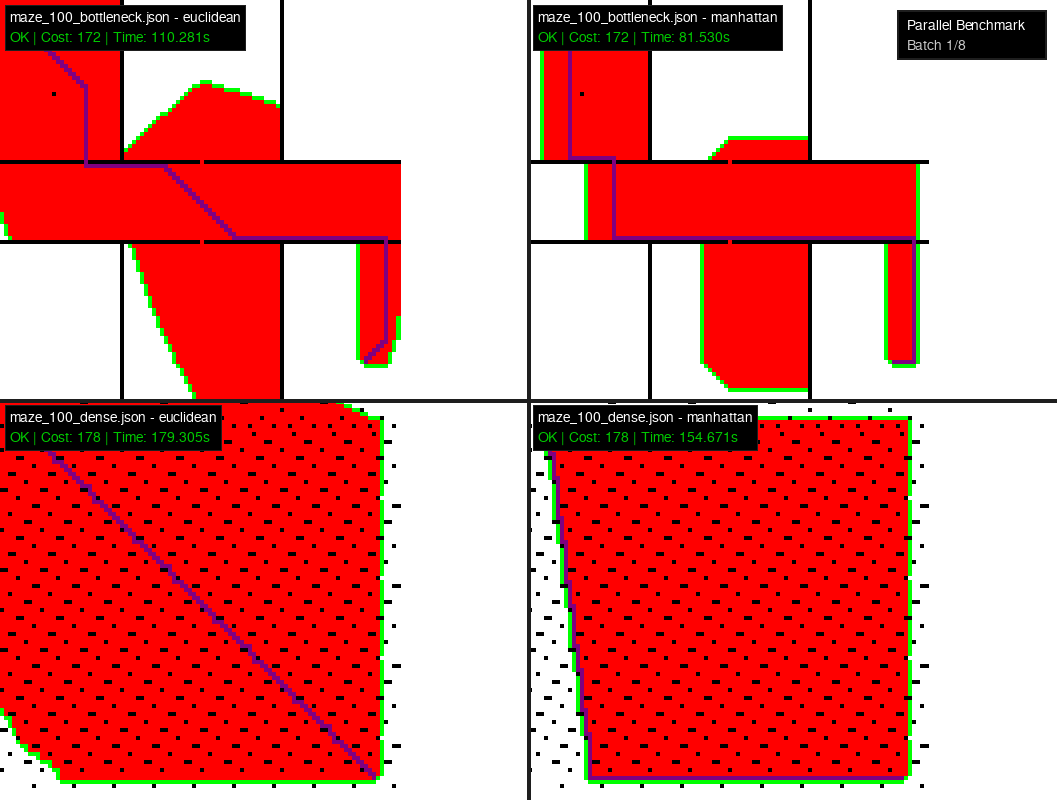
\includegraphics[width=0.45\textwidth]{screenshots/benchmark_batch_1_20251218_104500.png} &
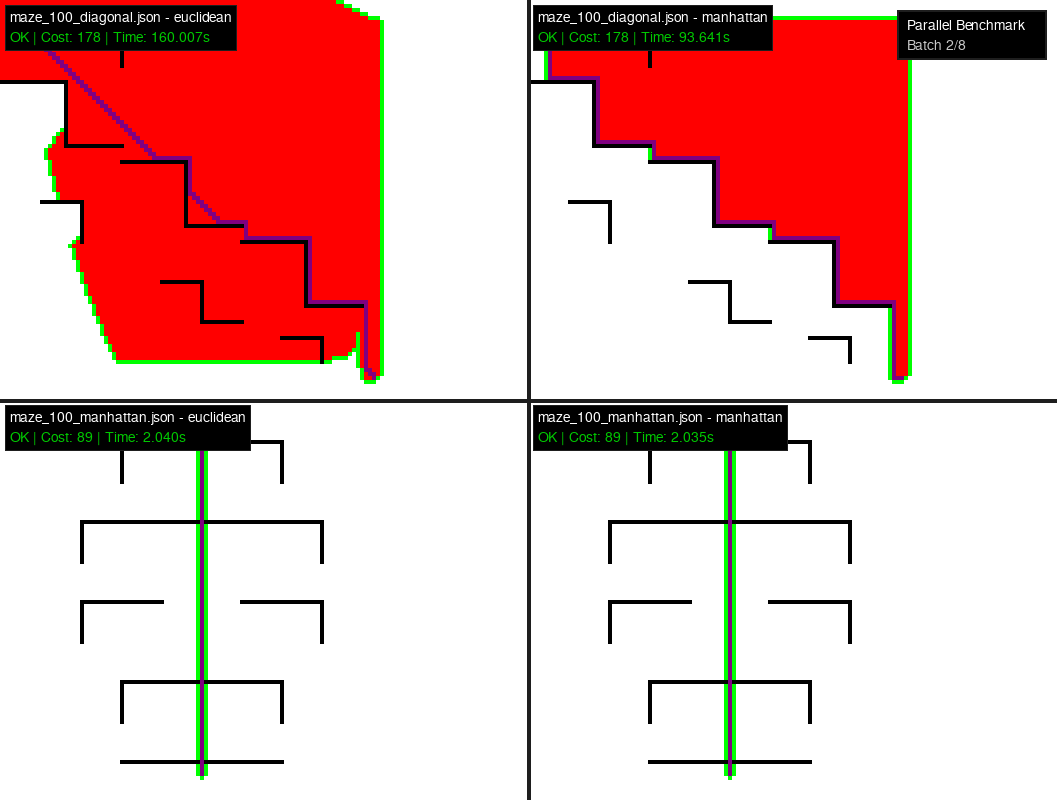
\includegraphics[width=0.45\textwidth]{screenshots/benchmark_batch_2_20251218_104741.png} \\
(a) Batch 1 & (b) Batch 2 \\[6pt]
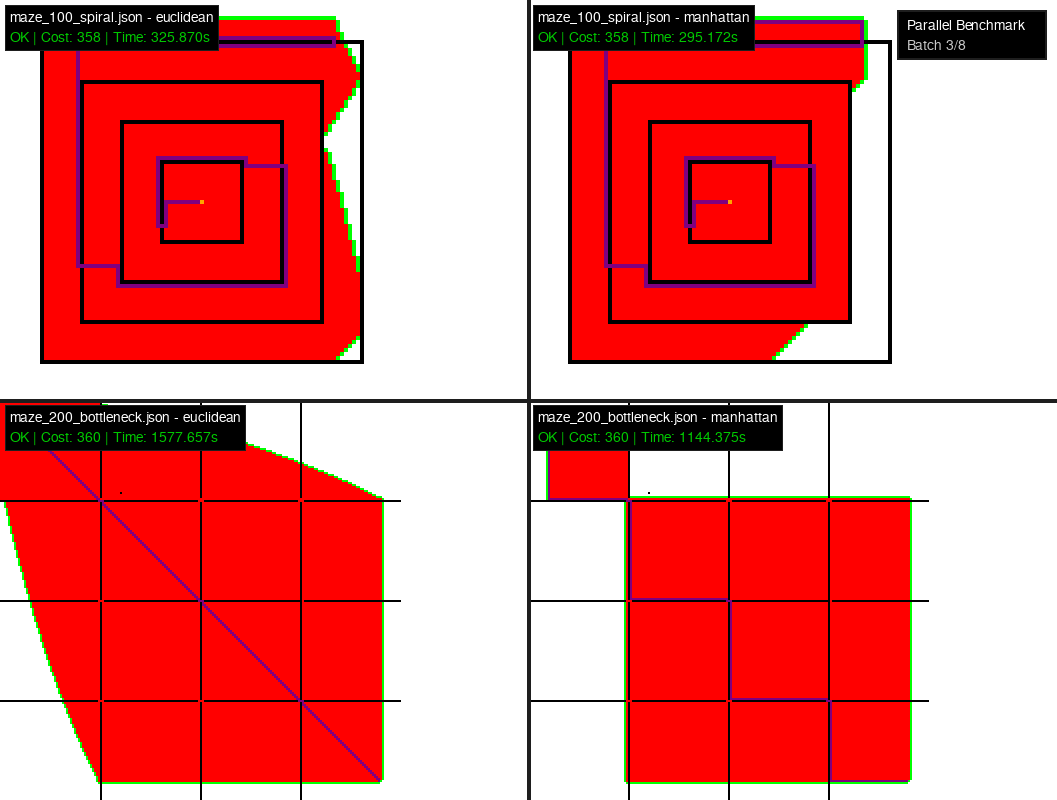
\includegraphics[width=0.45\textwidth]{screenshots/benchmark_batch_3_20251218_111401.png} &
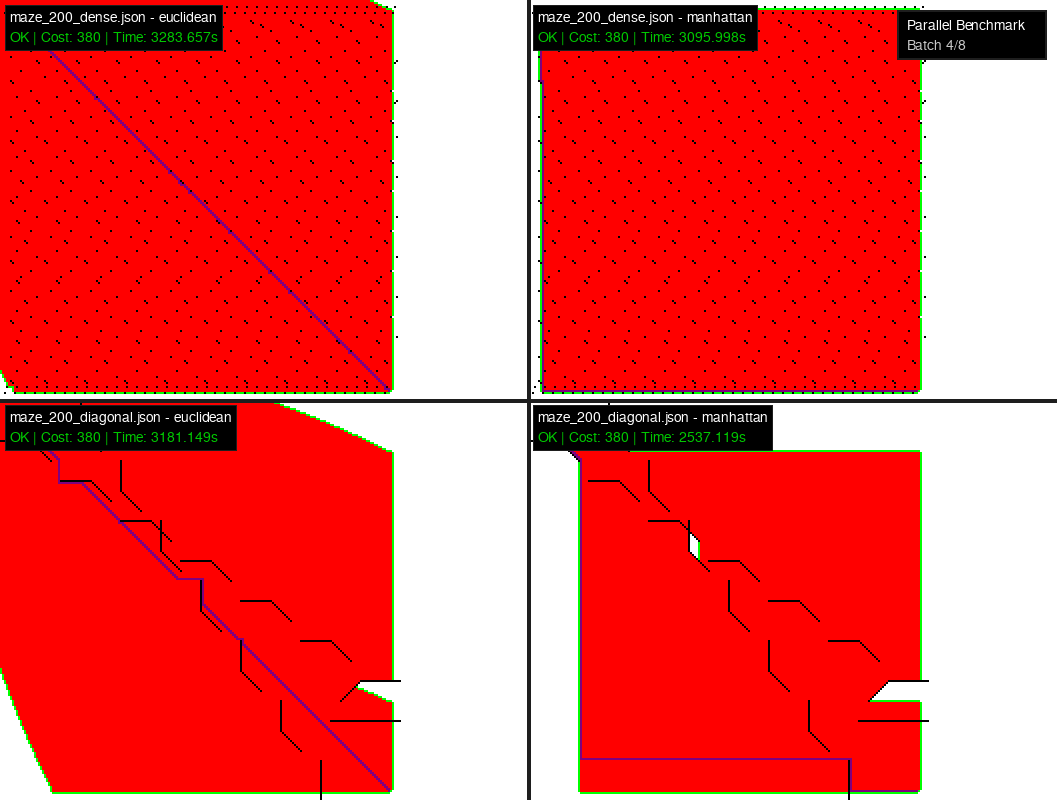
\includegraphics[width=0.45\textwidth]{screenshots/benchmark_batch_4_20251218_120846.png} \\
(c) Batch 3 & (d) Batch 4 \\
\end{tabular}
\caption{A* Pathfinding Visualizer: (a) Batch 1, (b) Batch 2, (c) Batch 3, (d) Batch 4}
\label{fig:visualization}
\end{figure}

\begin{figure}[ht]
\centering
\begin{tabular}{cc}
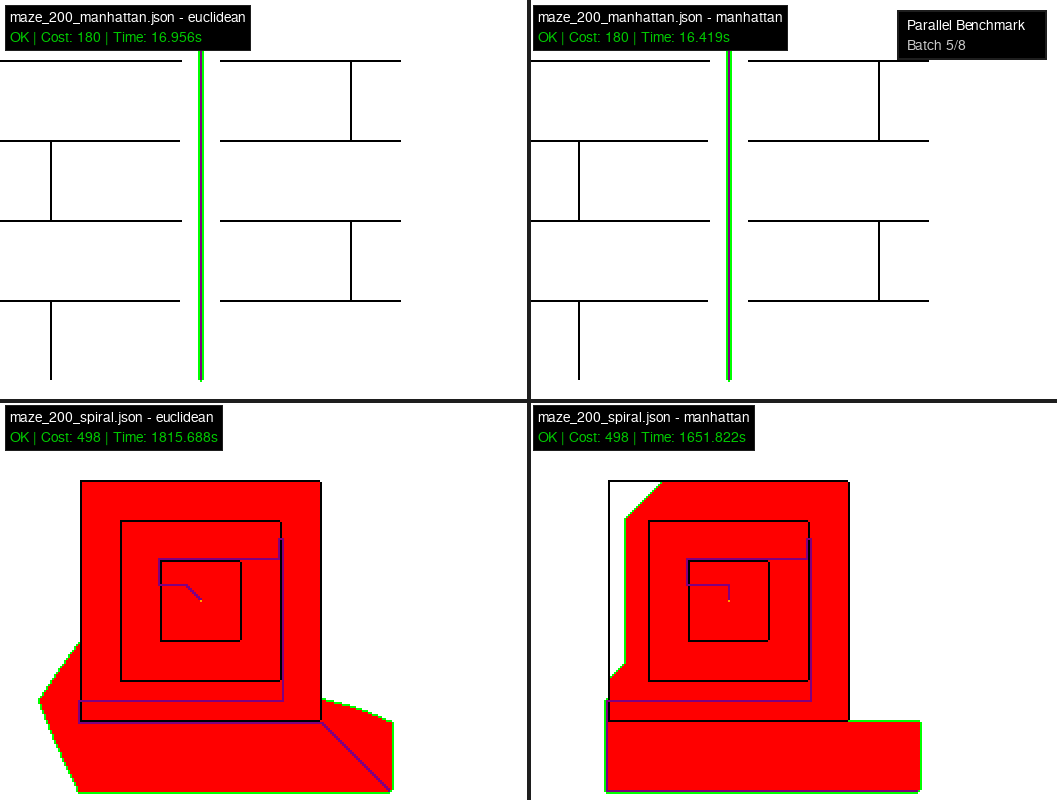
\includegraphics[width=0.45\textwidth]{screenshots/benchmark_batch_5_20251218_123904.png} &
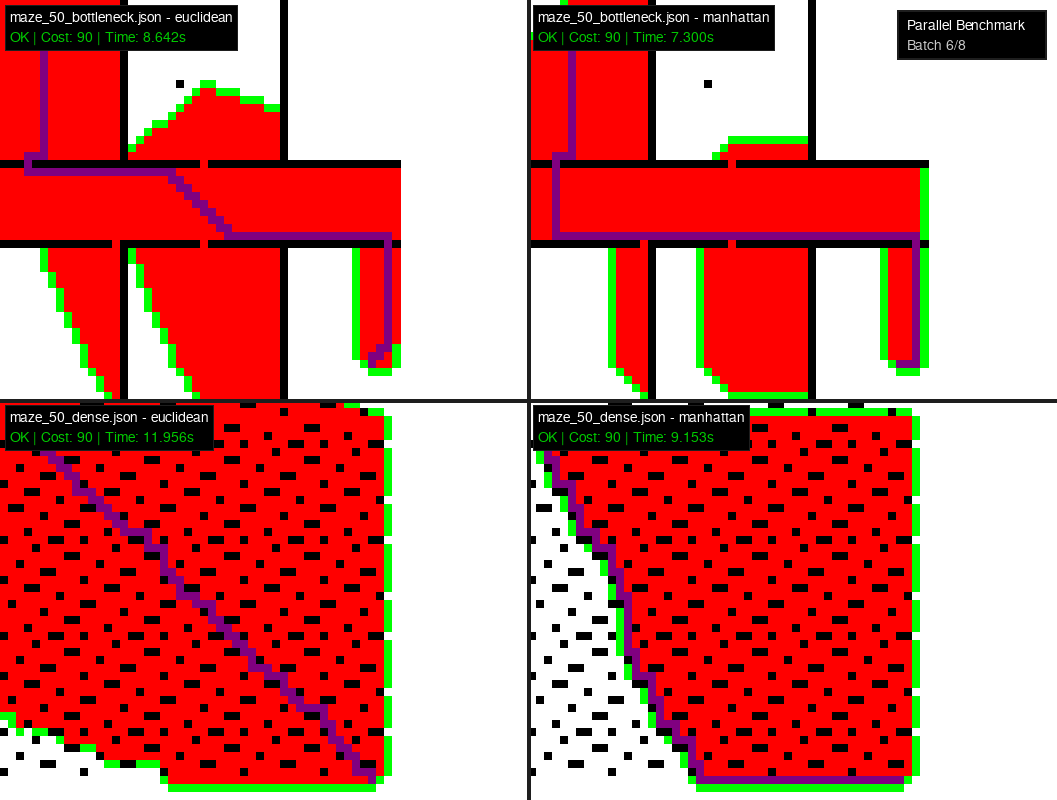
\includegraphics[width=0.45\textwidth]{screenshots/benchmark_batch_6_20251218_123918.png} \\
(a) Batch 5 & (b) Batch 6 \\[6pt]
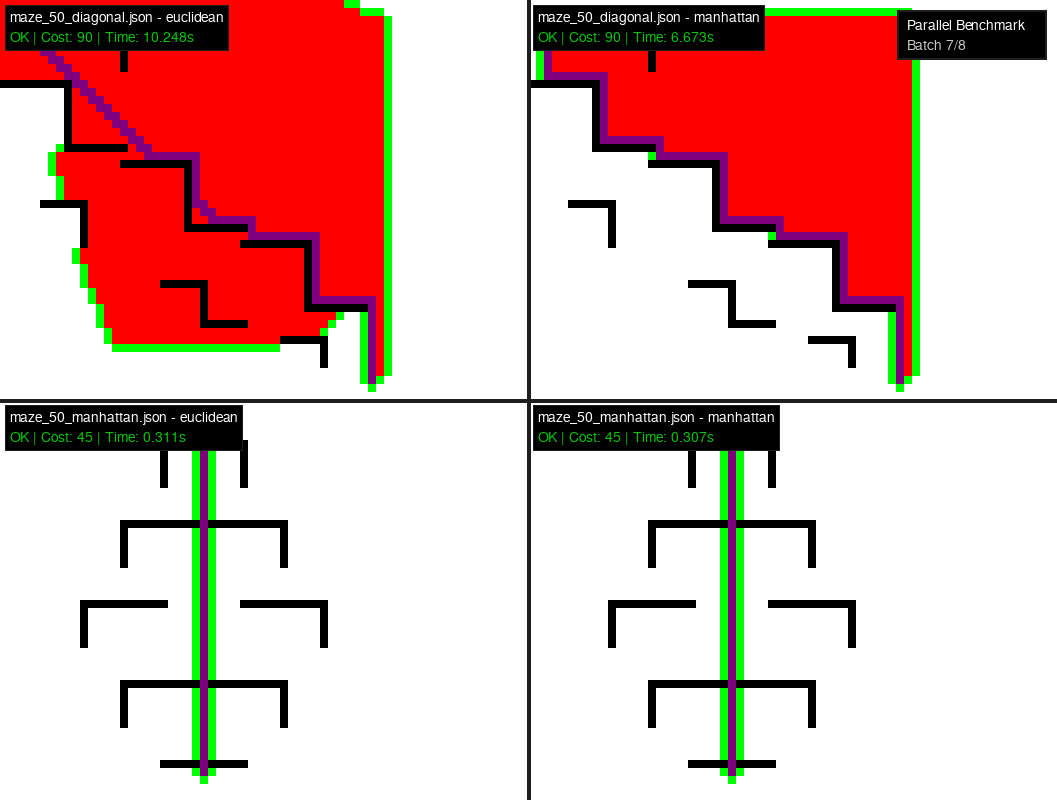
\includegraphics[width=0.45\textwidth]{screenshots/benchmark_batch_7_20251218_123930.png} &
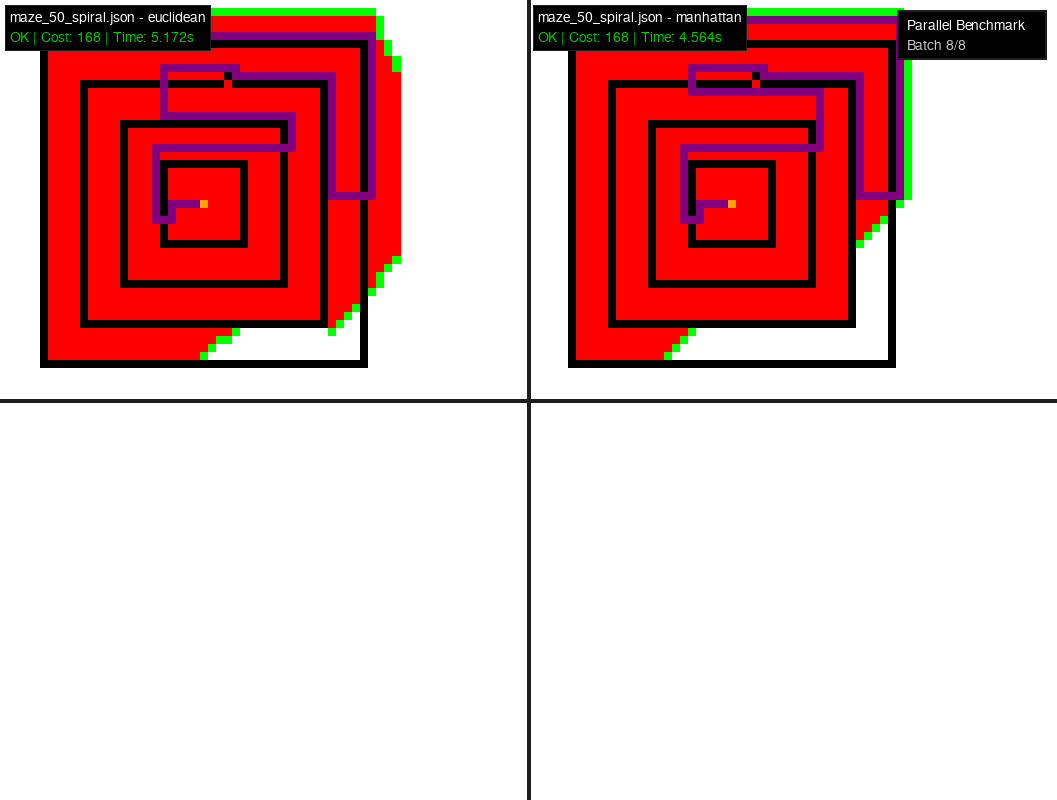
\includegraphics[width=0.45\textwidth]{screenshots/benchmark_batch_8_20251218_123936.png} \\
(c) Batch 7 & (d) Batch 8 \\
\end{tabular}
\caption{A* Pathfinding Visualizer: (a) Batch 5, (b) Batch 6, (c) Batch 7, (d) Batch 8}
\label{fig:visualization}
\end{figure}

\newpage
\section{Lessons and Experience}

\subsection{Programming Skills}

\subsubsection{Python Proficiency}
\begin{itemize}
    \item \textbf{OOP Design:} Design proper class structure for maintainability
    \item \textbf{Data Structures:} Use correct data structures (PriorityQueue, dict, set)
    \item \textbf{Performance Optimization:} Fast I/O, algorithm optimization
    \item \textbf{Libraries:} Proficient with pygame, pandas, matplotlib
\end{itemize}

\subsubsection{Algorithm Design}
\begin{itemize}
    \item Deep understanding of graph algorithms: A*, BFS, DFS, MST, Max Flow
    \item Know how to choose appropriate heuristic for problems
    \item Complexity analysis and optimization skills
    \item Trade-off between accuracy and performance
\end{itemize}

\subsection{Software Engineering}

\subsubsection{Project Structure}
\begin{itemize}
    \item Organize code into clear modules
    \item Separation of concerns: UI, algorithm, benchmark, analysis
    \item Documentation with detailed README.md
    \item Version control with Git
\end{itemize}

\subsubsection{Testing and Validation}
\begin{itemize}
    \item Design comprehensive test cases (15 mazes)
    \item Automated testing with benchmark system
    \item Validation with BFS to ensure correctness
    \item Performance metrics collection
\end{itemize}

\subsubsection{User Experience}
\begin{itemize}
    \item Interactive UI design with pygame
    \item Real-time feedback and visualization
    \item Multiple configuration options
    \item Clear documentation and instructions
\end{itemize}

\subsection{Problem Solving}

\subsubsection{Analytical Thinking}
\begin{itemize}
    \item \textbf{Identify bottlenecks:} Found I/O was the issue in HUSTACK, not algorithm
    \item \textbf{Research solutions:} Learn about Fast I/O techniques
    \item \textbf{Benchmark everything:} Measure before and after optimization
    \item \textbf{Data-driven decisions:} Choose heuristic based on benchmark results
\end{itemize}

\subsubsection{Debugging Skills}
\begin{itemize}
    \item Use print debugging effectively
    \item Check edge cases and corner cases
    \item Validation with known-correct algorithms (BFS)
    \item Step-by-step verification in visualization
\end{itemize}

\subsection{Research and Self-Learning}

\subsubsection{Learning Resources}
During the project, I used many resources:
\begin{itemize}
    \item A* Algorithm: Wikipedia, GeeksforGeeks
    \item Pygame documentation and tutorials
    \item Competitive programming blogs for Fast I/O
    \item Stack Overflow for specific problems
    \item Academic papers on pathfinding algorithms
\end{itemize}

\subsubsection{Continuous Improvement}
\begin{itemize}
    \item Constantly refactor code to improve readability
    \item Add features based on feedback and ideas
    \item Optimize performance when discovering bottlenecks
    \item Document lessons learned
\end{itemize}

\subsection{Time Management}

\subsubsection{8-week Project Timeline}
\begin{enumerate}
    \item \textbf{Week 1-2:} Research A*, design architecture
    \item \textbf{Week 3-4:} Implement core algorithm and basic UI
    \item \textbf{Week 5-6:} Add features (themes, save/load, random maze)
    \item \textbf{Week 7:} Benchmark system and test mazes
    \item \textbf{Week 8:} Analysis tools, documentation, final polish
\end{enumerate}

\subsubsection{Lessons Learned}
\begin{itemize}
    \item \textbf{Start early:} Have enough time to research and iterate
    \item \textbf{Incremental development:} Build one feature at a time, test thoroughly before next
    \item \textbf{Document as you go:} Write README and comments immediately, don't leave for last
    \item \textbf{Buffer time:} Reserve time for debugging and unexpected issues
\end{itemize}

\subsection{Key Takeaways}

\subsubsection{Technical Skills}
\begin{enumerate}
    \item \textbf{Algorithm mastery:} Deep understanding of DSA is not just memorizing theory
    \item \textbf{Optimization matters:} I/O optimization as important as algorithm
    \item \textbf{Right tool for the job:} Choosing appropriate data structure is crucial
    \item \textbf{Testing is crucial:} Validation and benchmarking necessary for quality
\end{enumerate}

\subsubsection{Soft Skills}
\begin{enumerate}
    \item \textbf{Patience:} Debugging and optimization take time
    \item \textbf{Persistence:} Don't give up when facing TLE or bugs
    \item \textbf{Curiosity:} Learn deeper than required knowledge
    \item \textbf{Documentation:} Good documentation helps others and future self
\end{enumerate}

\newpage
\section{Conclusion and Future Development}

\subsection{Summary}
Project 1 course brought me:

\subsubsection{Knowledge}
\begin{itemize}
    \item Master data structures: Tree, Graph, Hash Table, Stack, Queue
    \item Deep understanding of algorithms: Backtracking, DFS/BFS, MST, Max Flow, A*
    \item Optimization skills: Fast I/O, algorithm optimization, performance tuning
    \item Practical experience with project development from design to deployment
\end{itemize}

\subsubsection{Skills}
\begin{itemize}
    \item Python programming: from basic to advanced techniques
    \item Software engineering: project structure, testing, documentation
    \item Problem solving: analytical thinking, debugging, optimization
    \item Research: self-learning, finding resources, applying to practice
\end{itemize}

\subsection{Achievements}

\subsubsection{HUSTACK (Part 1)}
\begin{itemize}
    \item Completed 7 DSA topics
    \item Solved many exercises with increasing difficulty
    \item Discovered and applied Fast I/O optimization
    \item Improved performance by 10x for Python code
\end{itemize}

\subsubsection{A* Pathfinding Project (Part 2)}
\begin{itemize}
    \item Complete project with 1,336 lines of main code
    \item Interactive UI with pygame
    \item 15 test mazes covering diverse patterns
    \item Comprehensive benchmark system
    \item Analysis and visualization tools
    \item Detailed documentation with README.md
\end{itemize}

\subsection{Future Development}

\subsubsection{Improvements for Current Project}
\begin{enumerate}
    \item \textbf{Add algorithms:} Dijkstra, Bellman-Ford, Jump Point Search
    \item \textbf{Weighted edges:} Support terrain with different costs
    \item \textbf{3D visualization:} Extend to 3D pathfinding
    \item \textbf{CLI interface:} Command line tool for batch processing
    \item \textbf{Web version:} Port to web with JavaScript or Pygame Web
    \item \textbf{Machine Learning:} Learn heuristic function from data
\end{enumerate}

\subsubsection{Real-world Applications}
A* is widely used in:
\begin{itemize}
    \item \textbf{Game development:} NPC pathfinding, navigation mesh
    \item \textbf{Robotics:} Robot navigation, motion planning
    \item \textbf{GPS navigation:} Route planning with real-world constraints
    \item \textbf{Network routing:} Finding optimal path in networks
\end{itemize}

\subsubsection{Extended Knowledge}
For further development, I can learn:
\begin{itemize}
    \item \textbf{Advanced pathfinding:} Hierarchical A*, Any-angle pathfinding
    \item \textbf{Optimization algorithms:} Genetic algorithms, Simulated annealing
    \item \textbf{AI planning:} STRIPS, HTN planning
    \item \textbf{Computer graphics:} Rendering, collision detection
\end{itemize}

\subsection{Final Words}
Project 1 course not only helped me consolidate knowledge of Data Structures and Algorithms, but also developed programming skills, problem-solving thinking, and self-learning ability. From solving HUSTACK exercises with Fast I/O optimization, to building a complete A* Pathfinding project, each phase brought valuable lessons.

The A* Pathfinding Visualizer project gave me the opportunity to apply theory to practice, from basic algorithms to complex systems with UI, benchmark, and analysis tools. Benchmark results demonstrate deep understanding of algorithms and ability to scientifically evaluate performance.

I believe the knowledge and skills gained from this course will be a solid foundation for future projects and work, especially in software development and artificial intelligence fields.

\end{document}
